\documentclass{article}

\usepackage{amsmath}
\usepackage{graphicx}

\title{Fresnel integrals}
\author{Marco Majland}
\begin{document}
	\maketitle
	\noindent
	The Fresnel integrals are defined as
	\begin{equation}
		S(x) = \int_{0}^{x}\sin\Big(\frac{\pi t^2}{2}\Big)dt\quad\textrm{and}\quad C(x) = \int_{0}^{x}\cos\Big(\frac{\pi t^2}{2}\Big)dt
		\label{eq:Fresnel_integrals}
	\end{equation}
	which are transcendental functions\footnote{A transcendental function is an analytic function which does not satisfy a polynomial equation (as opposed to algebraic functions)}. They are related to Fresnel diffraction in classical optics. In order to investigate the properties of these integrals, they will in the following be calculated numerically using a numerical integration routine in C\# and compared to tabulated values given in https://www.dwc.knaw.nl/DL/publications/PU00011466.pdf. The tabulated values in X are calculated using the power series expansion of \ref{eq:Fresnel_integrals} which are given by
	\begin{equation}
		S(x) = \int_{0}^{x}\sin\Big(\frac{\pi t^2}{2}\Big)dt = \sum_{n = 0}^{\infty}(-1)^{n}\frac{x^{4n+3}}{(2n+1)!(4n+3)}
	\end{equation}
	and
	\begin{equation}
	C(x) = \int_{0}^{x}\cos\Big(\frac{\pi t^2}{2}\Big)dt = \sum_{n = 0}^{\infty}(-1)^{n}\frac{x^{4n+1}}{(2n)!(4n+1)}.
	\end{equation}
	The result of the numerical integration is presented in figure \ref{fig:integration}.
	\begin{figure}
	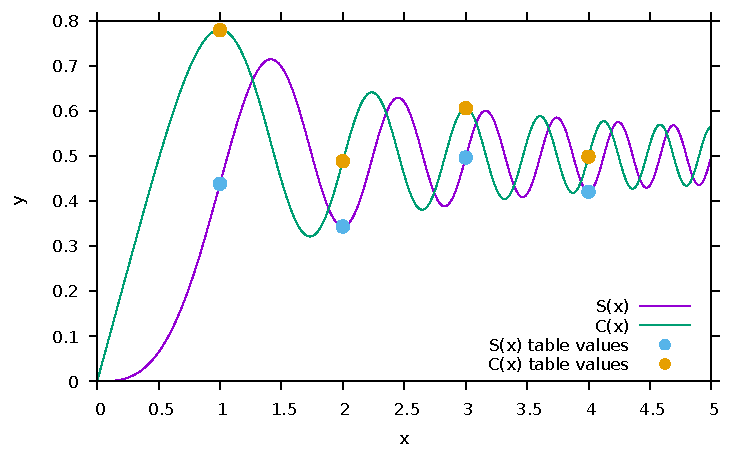
\includegraphics[]{Output.pdf}
	\caption{Numerical integration of the Fresnel integrals given by equation \ref{eq:Fresnel_integrals} along with the tabulated values given by REFERENCE.}
	\label{fig:integration}
	\end{figure}
	Analytically, equation \ref{eq:Fresnel_integrals} may be shown to converge to 1/2 in the limit $x\rightarrow\infty$. To test convergence, the numerical integration was made for higher values of x as depicted in figure \ref{fig:convergence}. Issues of the numerical integration routine are clearly seen in the intervals $x\in[18,21]$, $x\in[22,30]$ and $x\in[37,47]$. Otherwise, the integrals seem to converge for all other values of $x$ to $1/2$. Since the test of convergence is not made for $x = \textrm{machine infinity}$, it is not very indicative.
	\begin{figure}
	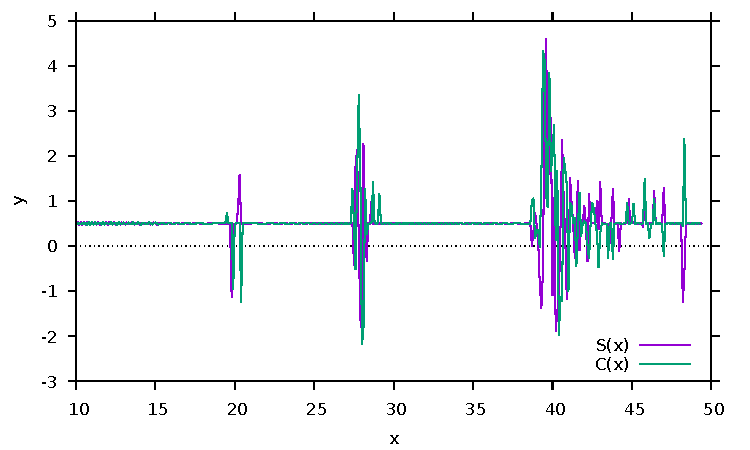
\includegraphics[]{Output2.pdf}
	\caption{Large values of $x$ in numerical integration of equation \ref{eq:Fresnel_integrals} to test convergence toward $1/2$.}
	\label{fig:convergence}
	\end{figure}	
\end{document}
